%SI 2014-09-05

\documentclass{article}

\usepackage[T1]{fontenc}
\usepackage[utf8]{inputenc}
\usepackage[swedish]{babel}
\usepackage{fullpage}
\usepackage{amssymb}
\usepackage{bussproofs}
\usepackage{amsmath}
\usepackage{graphicx}
\usepackage{verbatim}
\usepackage{tikz}

\usepackage{tkz-berge}
\let\emptyset\varnothing



\title{Supplemental Instructions}
\author{Benjamin Eriksson \& Erik Thorsell \\ 
		\small{beneri@student.chalmers.se} \&
		\small{erithor@student.chalmers.se}
}

\date{
     2014-12-16 
 }

\begin{document}
\maketitle

\subsection*{1}
Låt 
$
A = \frac{1}{2}
\begin{pmatrix}
	1 & -3 \\
	-3 & 1 
\end{pmatrix}
$
\begin{itemize}
\item[a) ] Bestäm alla egenvärden och egenvektorer till A.
\item[b) ] Beräkna $A^{1000}$
\end{itemize}

\subsection*{2}
Bestäm koordinaterna i standardbasen för den vektor $v \in \mathbb{R}^3$ som i basen \\ $F = (1 \quad 0 \quad 2)^t, (3 \quad 2 \quad 1)^t, (4 \quad 2 \quad -1)^t$ har koordinatvektorn $\mathbf{v}_{F} = (-1 \quad 2 \quad 1)^t$
\subsection*{3}
Ange grannmatrisen G för grafen nedan. Ange även övergångsmatrisen M för slumpvandringen på grafen.
\\
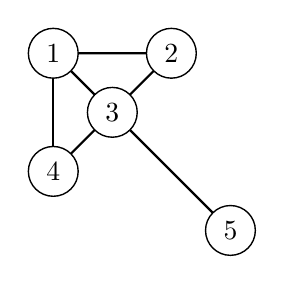
\begin{tikzpicture}[scale=0.75]
  \Vertex[x=0,y=4]{1}
  \Vertex[x=2,y=4]{2}
  \Vertex[x=1,y=3]{3}
  \Vertex[x=0,y=2]{4}
  \Vertex[x=3,y=1]{5}
  \tikzstyle{LabelStyle}=[fill=white,sloped]
  \tikzstyle{EdgeStyle}=[]
  \Edge[](1)(2)
  \Edge[](1)(3)
  \Edge[](1)(4)
  \Edge[](2)(3)
  \Edge[](3)(4)
  \Edge[](3)(5)
\end{tikzpicture}

\subsection*{4}
Bestäm (minsta) avståndet från punkten $P = (2,1,0)$ till linjen
\begin{equation}
    \begin{cases}
        x = 3 + t \\
        y = 4 + 2t \\
        z = 5 + 3t \\
    \end{cases}
\end{equation}

\subsection*{5}
Bestäm matrisen (i standardbasen) för den linjära avbildningen i $\mathbb{R}^2$ 
som består av spegling i linjen $y=-x$ följt av rotation $\frac{\pi}{6}$ radianer 
{\it moturs}.

\subsection*{6}
Låt $a$ vara ett reellt tal och sätt
$$
\vec{v_{1}} = 
\begin{pmatrix}
    2 \\
    -1 \\
    a \\
    0 \\
\end{pmatrix}
,
\vec{v_{2}} = 
\begin{pmatrix}
    1 \\
    3 \\
    2 \\
    1 \\
\end{pmatrix}
,
\vec{v_{3}} = 
\begin{pmatrix}
    1 \\
    -4 \\
    1 \\
    -1 \\
\end{pmatrix}
$$
\noindent
a) Bestäm, för varje värde på $a$, alla lösningar till ekvatationssystemet:
$$ x_{1} \vec{v_{1}} + x_{2} \vec{v_{2}} + x_{3} \vec{v_{3}} = 0 $$
b) Avgör för vilka $a$ vektorerna $\vec{v_{1}}, \vec{v_{2}}$ och $\vec{v_{3}}$ 
är linjärt obereonde.

\end{document}
